%% ----------------------------------------------------------------
%% Thesis.tex -- MAIN FILE (the one that you compile with LaTeX)
%% ---------------------------------------------------------------- 

% Set up the document
\documentclass[a4paper, 11pt, oneside]{Thesis}  % Use the "Thesis" style, based on the ECS Thesis style by Steve Gunn
\graphicspath{Figures/}  % Location of the graphics files (set up for graphics to be in PDF format)

% Include any extra LaTeX packages required
\usepackage[square, numbers, comma, sort&compress]{natbib}  % Use the "Natbib" style for the references in the Bibliography
\usepackage{verbatim}  % Needed for the "comment" environment to make LaTeX comments
\usepackage{vector}  % Allows "\bvec{}" and "\buvec{}" for "blackboard" style bold vectors in maths
\hypersetup{urlcolor=blue, colorlinks=true}  % Colours hyperlinks in blue, but this can be distracting if there are many links.
\usepackage{graphicx}
\usepackage[dutch]{babel}

%% ----------------------------------------------------------------
\begin{document}
\frontmatter      % Begin Roman style (i, ii, iii, iv...) page numbering

% Set up the Title Page
\title  {Stadslab FabTool}
\authors  {
	Marcelo Dias Avelino \\
	Nilson Xavier da Luz
}
\addresses  {\groupname \\ \deptname \\ \univname}  % Do not change this here, instead these must be set in the "Thesis.cls" file, please look through it instead
\date       {\today}
\subject    {}
\keywords   {}

\maketitle
%% ----------------------------------------------------------------

\setstretch{1.3}  % It is better to have smaller font and larger line spacing than the other way round

% Define the page headers using the FancyHdr package and set up for one-sided printing
\fancyhead{}  % Clears all page headers and footers
\rhead{\thepage}  % Sets the right side header to show the page number
\lhead{}  % Clears the left side page header

\pagestyle{fancy}  % Finally, use the "fancy" page style to implement the FancyHdr headers

%% ----------------------------------------------------------------
\lhead{\emph{FabTool}}  % Set the left side page header to "Contents"
\tableofcontents  % Write out the Table of Contents

%% ----------------------------------------------------------------
\mainmatter	  % Begin normal, numeric (1,2,3...) page numbering
\pagestyle{fancy}  % Return the page headers back to the "fancy" style

% Include the chapters of the thesis, as separate files
% Just uncomment the lines as you write the chapters

\chapter{Introductie}

Dit verslag is geschreven met betrekking tot het vak ICT-lab (TIRLAB01 en TIRLAB02). Het is een project aangeboden door het Stadslab Rotterdam. Het Stadslab is een initiatief van de Hogeschool Rotterdam en de Gemeente Rotterdam om iedereen een kans te bieden om met technische apparatuur te werken waar ze normaal geen toegang tot zouden hebben. De enige voorwaarde dat het Stadslab stelt voor het benutten van hun apparatuur is dat de kennis dat opgedaan tijdens het verblijf vrij wordt gegeven. Hierdoor kunnen  andere personen dat later aan hun eigen projecten gaan werken bij de Stadslab dezelfde kennis gebruiken. Deze kennis kan in vele vormen voorkomen, maar de meest belangrijke zijn de gebruikte instellingen van de benutigde apparatuur. Dit omdat het uittesten van verschillende instellingen heel veel tijd kan kosten zonder een uitgangspunt.


De doelen van dit project zijn als volgt:
\begin {itemize}
\item Het delen van kennis zo simpel, snel en makkelijk mogelijk te maken.
\item Het doorzoekbaar maken van de gedeelde informatie.	
\item Een overzicht cre\"eren van het aantal bezoeken en welke apparaten zijn gebruikt in een bepaalde aanpasbare periode.
\item Het project goed documenteren zodat andere ontwikkelaars er met zo min mogelijk moeite verder aan kunnen werken.
\end {itemize} % Introduction

\chapter{Architectuur}

Het systeem is ontworpen en ge\"implementeerd in de vorm van een webapplicatie omdat het overal makkelijk te bereiken is en werkt op elke systeem met een webbrowser. De applicatie is verdeeld in meerdere onderdelen en elke onderdeel zal besproken worden in deze hoofdstuk.

\section{Checkins en checkouts}

\'E\'en van de onderdelen van de applicatie is de checkins en checkouts gedeelte. Dit gedeelte wordt gebruik om gebruikers de mogelijkheid te geven om in te checken als ze binnen komen en uit te checken als ze het lab verlaten.

\subsection{Checkin}

Als iemand het lab wilt gebruiken, worden ze verzocht om bij de ingang van het Stadslab in te checken. Het inchecken bestaat uit persoonlijk informatie en de doel van het bezoek invullen. De informatie die ingevuld moet worden verschilt per de volgende categori\"en: Student, Bedrijf en Overige.

\subsection{Checkout}

Nadat iemand zijn project heeft afgerond, wordt van diegene dan verwacht om uit te checken voor het verlaten van het lab. Bij het uitchecken moet de gebruiker informatie delen over waarmee en hoe het project is gemaakt.

\ % Architecture 

\chapter{Technologi\"en}

Wij hebben gekozen voor de volgende technologi\"en voor het ontwikkelen van deze webapplicatie:
\begin{itemize}
	\item Groovy - Een dynamische en behendig object geori\"enterd taal gebaseerd op de taal Java.
	\vspace{2mm} \\
	\textit{Wij hebben hiervoor gekozen omdat Java niet de meest prettig taal is om mee te ontwikkelen maar de Java Virtual Machine, waar Groovy ook op draait, heel stabiel en veilig is. Groovy maakt gebruikt van de sterkte punten van Java en verbetert de tekorkommingen.}

	\item Grails - Een webframework voor Groovy met de motto ``Convention over configuration''. Het is gefocused op het snel en makkelijk opzetten van webapplicaties.
	\vspace{2mm} \\
	\textit{Wij hebben hiervoor gekozen omdat dit het best ontwikkeld en langst bestand webframework is voor Groovy. Hun ontwikkelings filosofie maakte het ons ook makkelijk om een werkend webapplicatie te maken binnen beperkt tijd.}

	\item Vaadin - Een framework om moderne graphical user interfaces voor webapplicaties te bouwen.
	\vspace{2mm} \\
	\textit{Wij hebben hiervoor gekozen omdat Vaadin het makkelijk maakt om interfaces te maken en tegelijke tijd alle controle over te houden.}
\end{itemize} % Technology

\chapter{Implementatie}

\section{Checkin}

Als de gebruiker het lab binnen loopt, moet hij eerst inchecken. Om dat mogelijk te maken is een apart pagina gemaakt. Deze pagina is in 
Figuur \ref{fig:checkinoutview} te zien. Het bestaat uit 3 hoofdcomponenten: het welkomsbericht, de checkin knoppen en de checkout tabel.

\begin{figure}[Hh]
	\centering
	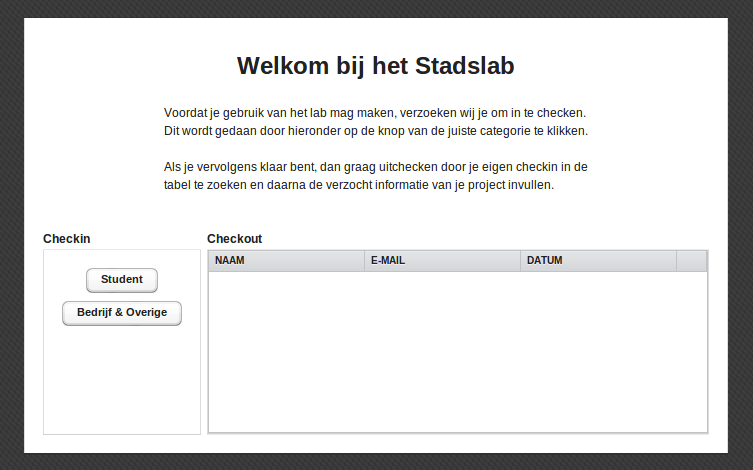
\includegraphics[width=\textwidth]{Images/checkinoutview2.png}
	\caption{Venster waar kan worden ingecheckt en uitgecheckt}
	\label{fig:checkinoutview}
\end{figure}

Het welkomsbericht bestaat uit een korte stuk tekst waarin uitgelegd wordt wat de bedoeling van deze pagina is. \\
Daaronder staan de checkin knoppen. Gebruikers horen de knop te kiezen dat bij hun past, als student of bedrijf/overige zijnde.\\ 

\subsection{Student}

Als een student in wilt checken, dan krijgt de student een venster te zien als weergegeven in Figuur \ref{fig:checkin-student}. Hierbij wordt persoonlijk informatie van de student gevraagd dat door de beheerders gebruikt wordt om bijvoorbeeld kosten te declareren bij de corresponderende instituut. Er wordt verder ook gevraagd met welke apparaten de student zal gaan werken. Hierdoor kunnen de beheerders een overzicht krijgen over welke apparaten de populairste zijn. Verder is er validatie ingebouwd om te zorgen dat alle velden ingevuld zijn, als afgebeeld in Figuur \ref{fig:checkin-student-error}. \\

\begin{figure}[Hh]
	\centering
	\subfigure[Checkin met ingevuld gegevens]{
		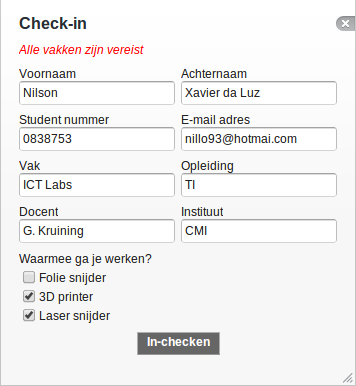
\includegraphics[width=175px, height=225px]{Images/checkin-student.png}
		\label{fig:checkin-student}
	}
	\subfigure[Checkin met errors]{
		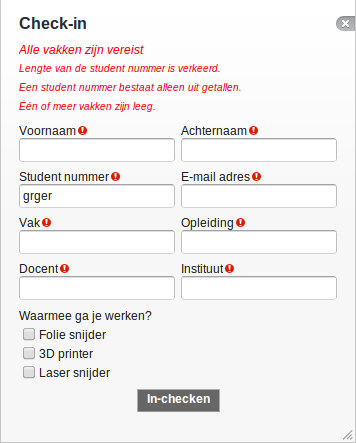
\includegraphics[width=175px, height=225px]{Images/checkin-student-error.png}
		\label{fig:checkin-student-error}
	}
	\caption{Checkin voor studenten}
\end{figure}

\subsection{Bedrijf en Overige}

Als een bedrijf of overige iemand in wilt checken dat krijgt diegene ook een eigen venster te zien. Hier wordt andere soort informatie gevraagd dat meer bij deze categorie past. Dit venster is te zien bij Figuur \ref{fig:checkin-company}. Ook hier wordt de ingevuld informatie gevalideerd om te zorgen dat alle informatie ingevuld is, dit is weergegeven in Figuur \ref{fig:checkin-company-error}. \\

\begin{figure}[Hh]
	\centering
	\subfigure[Checkin met ingevuld gegevens]{
		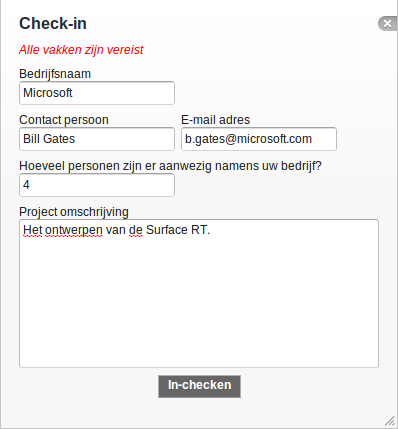
\includegraphics[width=175px, height=225px]{Images/checkin-company.png}
		\label{fig:checkin-company}
	}
	\subfigure[Checkin met errors]{
		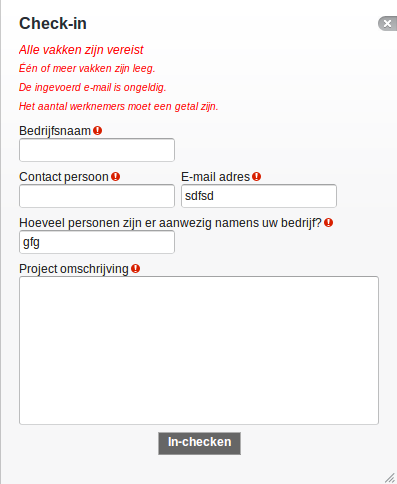
\includegraphics[width=175px, height=225px]{Images/checkin-company-error.png}
		\label{fig:checkin-company-error}
	}
	\caption{Checkin voor bedrijven}
\end{figure}

Zodra de gebruiker heeft ingecheckt, dan is de gebruiker vrij om gebruik te maken van het lab. Er komt dan een nieuwe element in de checkouts tabel te staan met de informatie van de gebruiker en een knop om uit te checken. Dit is te zien in Figuur \ref{fig:checkout-table}. \\

\begin{figure}[Hh]
	\centering
	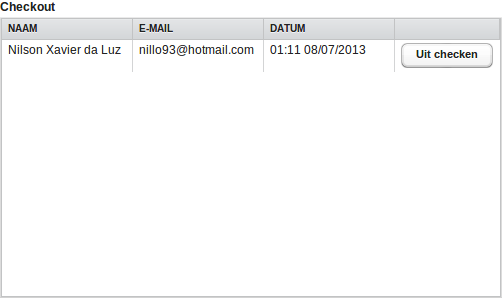
\includegraphics[width=0.65\textwidth]{Images/checkout-table.png}
	\caption{Pagina waar kan worden ingecheckt en uitgecheckt}
	\label{fig:checkout-table}
\end{figure}

\section{Checkout}

Wanneer de gebruiker klaar is en het lab wilt verlaten, wordt hij verzocht om eerste uit te checken. Dit gebeurt door zijn eigen informatie op te zoeken in de tabel en op de ``Uit checken'' knop te drukken. Er verschijnt dan een nieuwe venster om de benodigde informatie in te vullen over het project. Dit venster is weergegeven in Figuur \ref{fig:checkout-window}.

\begin{figure}[Hh]
	\centering
	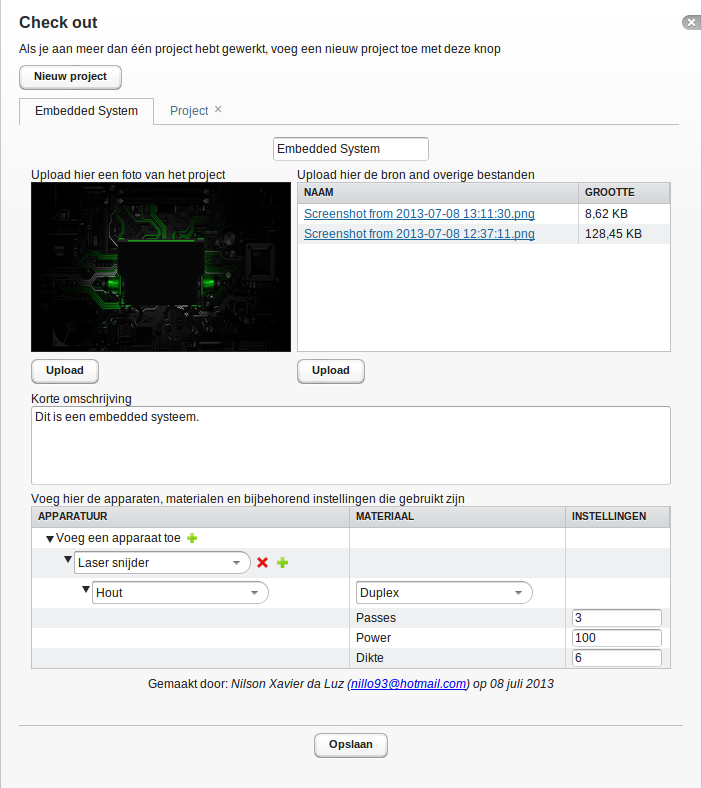
\includegraphics[width=0.65\textwidth]{Images/checkout-window.png}
	\caption{Venster waar kan worden uitgecheckt}
	\label{fig:checkout-window}
\end{figure}

Om te kunnen uitchecken wordt de volgende informatie gevraagd:

\subsection{Titel}

De titel wordt gebruikt om de project te identificeren. De titel moet uniek zijn.

\subsection{Foto}

Een foto van het project. Daarin moet duidelijk te zien zijn wat het project is.

\subsection{Bron bestanden}

Bron en overige bestanden van het project. Dit kan source code, 3D-modellen of iets anders zijn.

\subsection{Korte omschrijving}

Een korte omschrijving over wat het project is en/of doet.

\subsection{Instellingen}

Hier worden de gebruikte instellingen ingevuld van de gebruikte apparatten. Dit wordt gedaan door eerst apparaten toe te voegen, daarna materialen waaronder verschillende types te kiezen valt. Als een materiaal gekozen is, verschijnen de nodige instellingen van de gekozen apparaat en velden waar de instellingen kunnen worden ingevuld. \\

Er kunnen meerdere projecten worden aangemaakt voor het geval dat de gebruiker aan meerdere projecten heeft gewerkt. Dit wordt gedaan door op de ``Nieuw project'' knop dat bovenaan staat te drukken. Hierdoor wordt een nieuwe tab toegevoegd naast de tab van het bestaande project. \\
Als alles correct is ingevuld, dan wordt de checkout opgeslagen en is de gebruiker uitgecheckt.

\section{FabTool}

Het hoofdgedeelte van de webapplicatie is de FabTool, zie Figuur \ref{fig:fabtool}. Dit is waar projecten kunnen gezocht en bekeken, en waar beheerders overzicht kunnen houden over alle checkins, en apparaten kunnen beheren.

\begin{figure}[Hh]
	\centering
	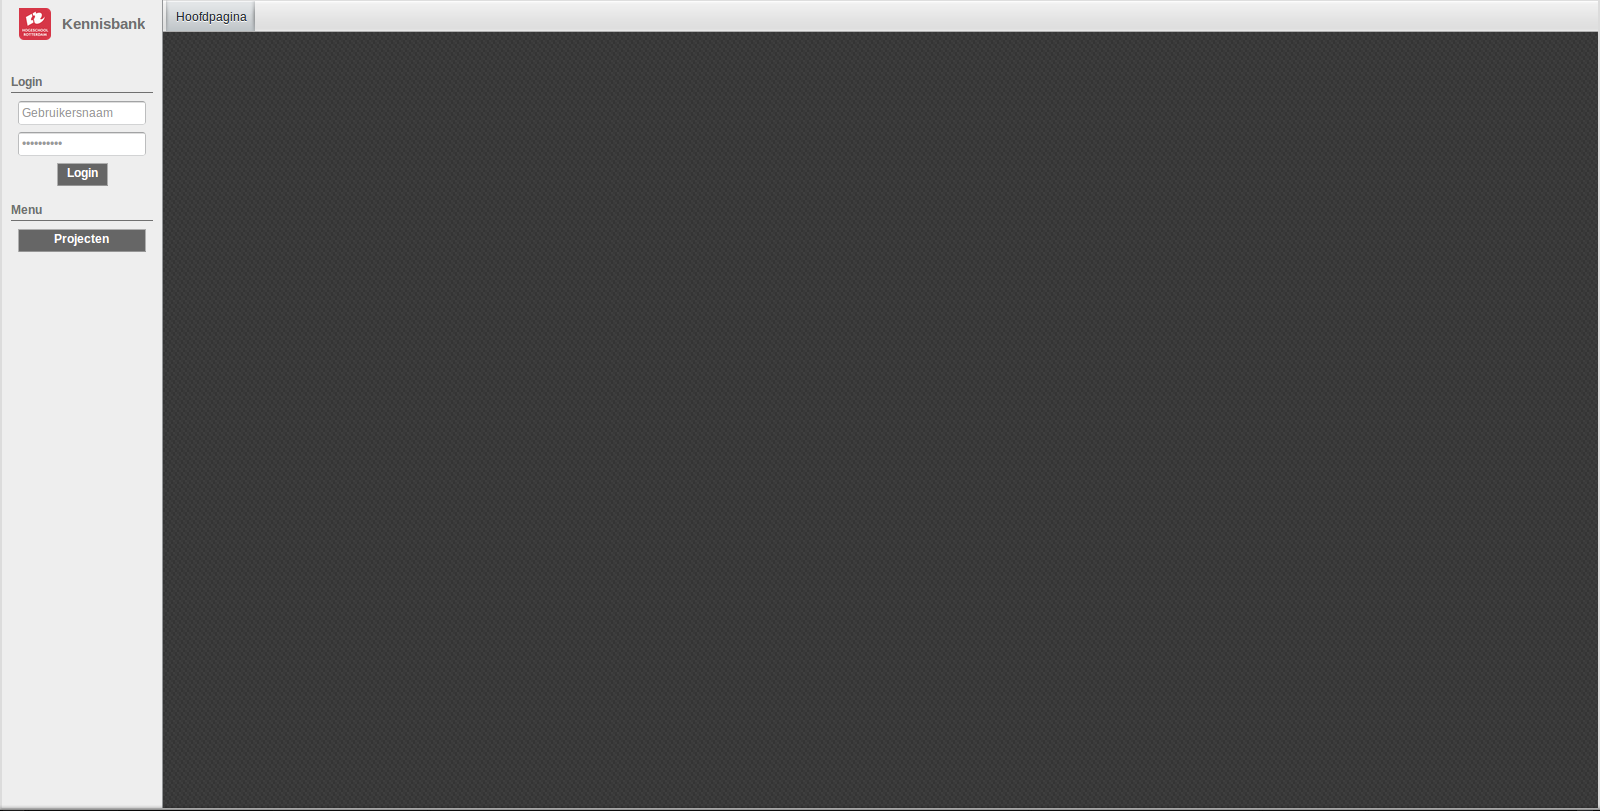
\includegraphics[width=1\textwidth]{Images/fabtool.png}
	\caption{Design van de FabTool}
	\label{fig:fabtool}
\end{figure}

\subsection{Projecten}

Een van de componenten van de FabTool is de projecten component. Hier worden alle projecten die tot nu toe zijn gemaakt weergegeven, zoals het te zien is op Figuur \ref{fig:projects}.

\begin{figure}[Hh]
	\centering
	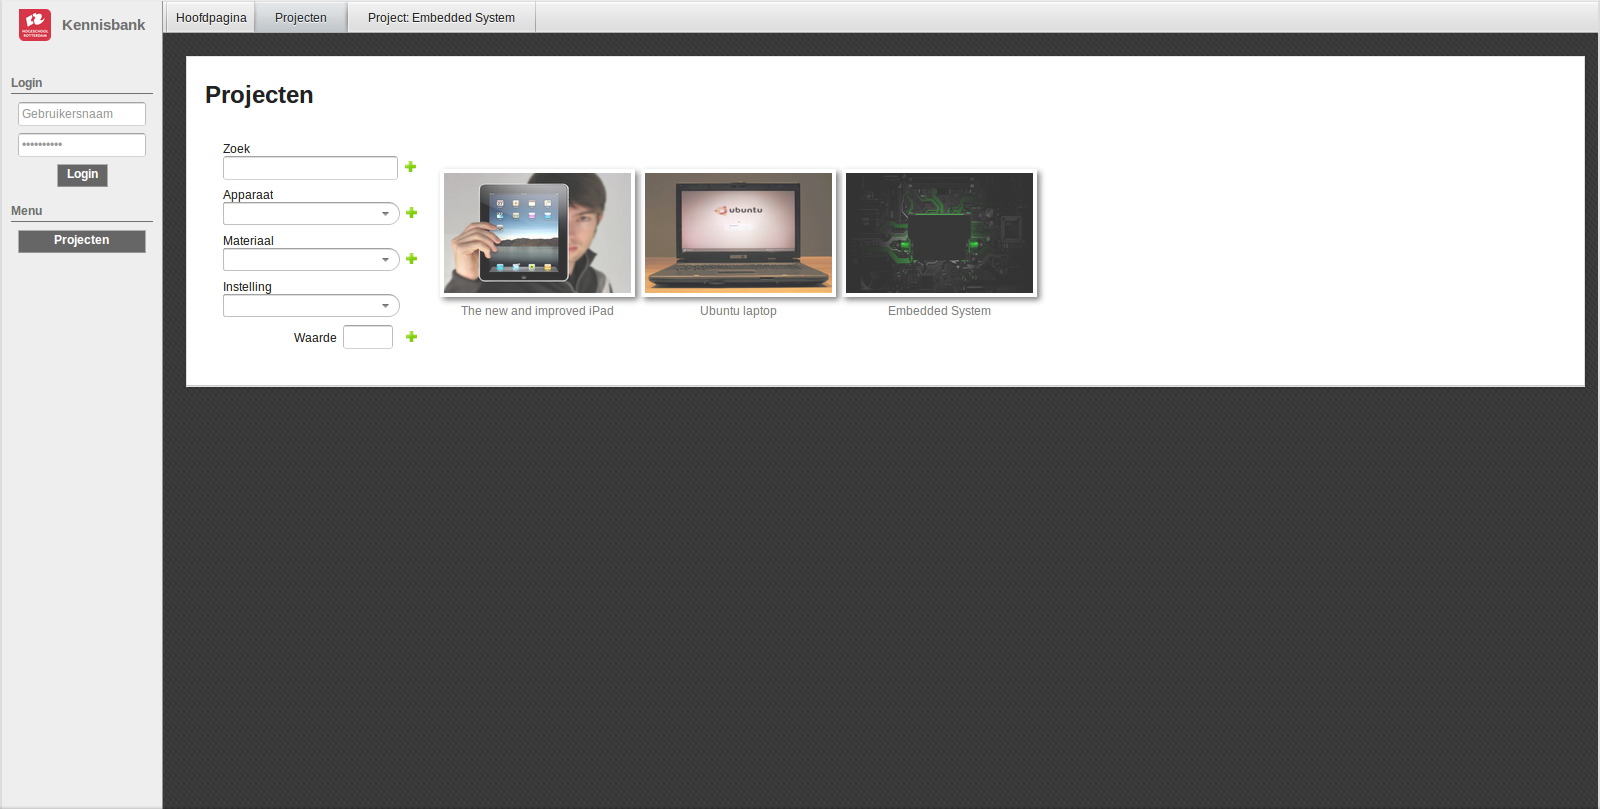
\includegraphics[width=1\textwidth]{Images/projects.png}
	\caption{Pagina waar projecten worden weergegeven}
	\label{fig:projects}
\end{figure}

Het geeft gebruikers ook de mogelijkheid om naar projecten te zoeken en uit te filteren. Zoals het is weergegeven is in Figuur \ref{fig:filter-projects}, kunnen project op meerdere categori\"en worden gefilterd. Ze kunnen per soort apparaat, materiaal en instelling worden gezocht. Ook is het mogelijk om naar tekst te zoeken dat in de titel of bij de omschrijving voorkomt.

\begin{figure}[Hh]
	\centering
	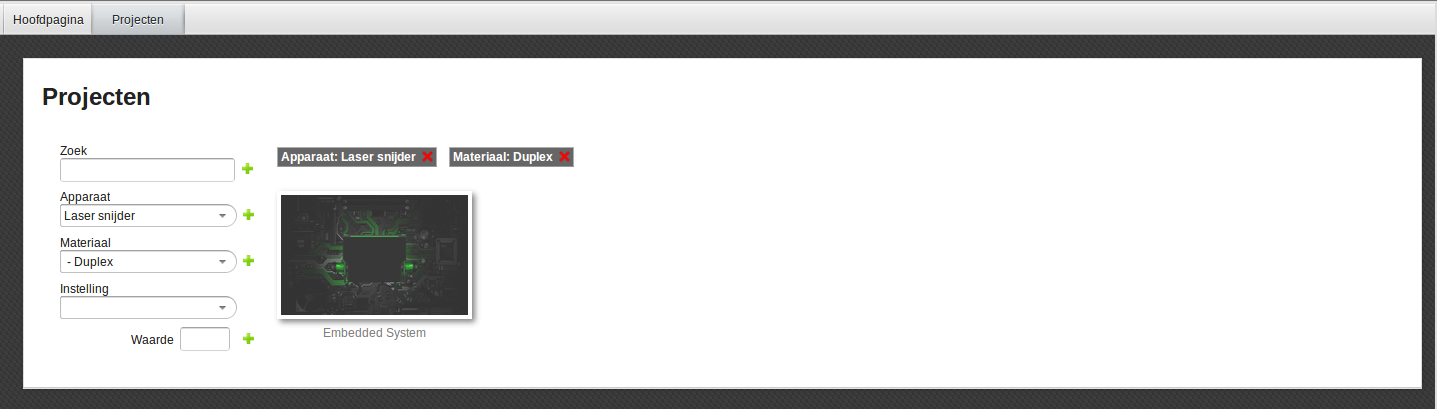
\includegraphics[width=1\textwidth]{Images/filter-projects.png}
	\caption{Projecten worden gefilterd}
	\label{fig:filter-projects}
\end{figure}

Als de gebruiker het project heeft gevonden waar hij naar zocht, kan hij erop klikken. Hierdoor verschijnt een nieuwe pagina met hetzelfde informatie dat tijdens het inchecken is ingevuld. Dit is te zien in Figuur \ref{fig:filter-projects}.

\begin{figure}[H]
	\centering
	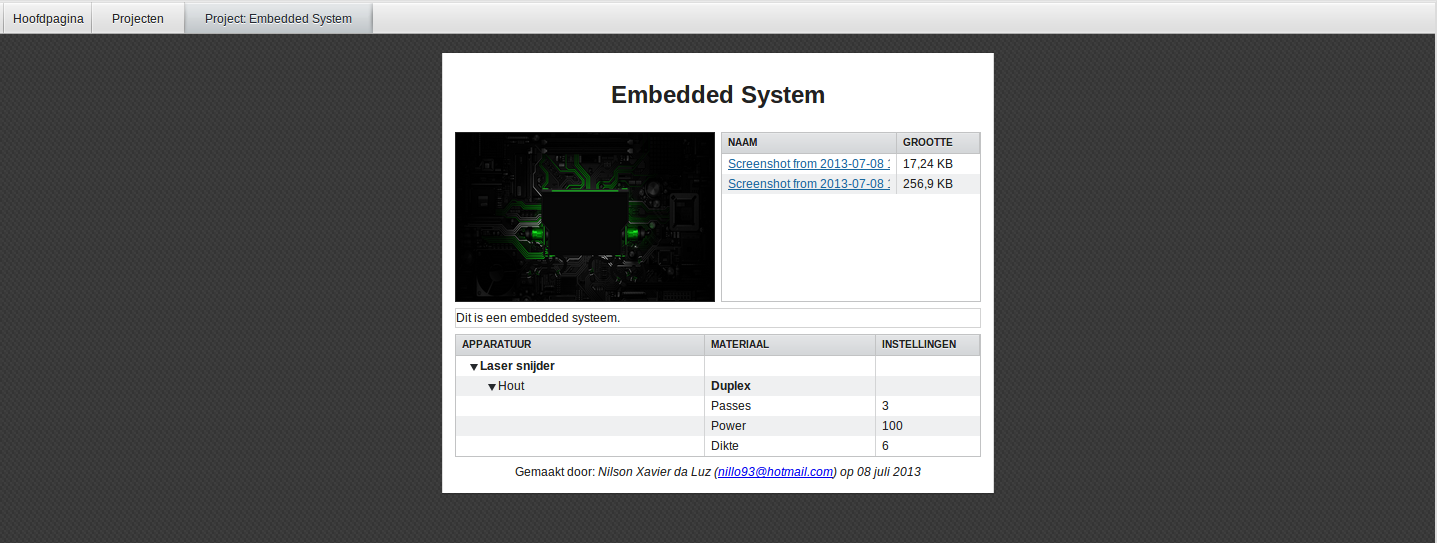
\includegraphics[width=1\textwidth]{Images/project.png}
	\caption{Gekozen project}
	\label{fig:filter-projects}
\end{figure}

\subsection{Administratie}
De Administratie is een page waar wordt bijgehouden wie er in de stadslab is geweest en wanneer. Dit is wordt gedaan door een tabel erin te maken met alle check-ins en mogelijkheid te geven om de check-ins te filteren om zo te zien in welke periode de druk was of juist rustig. Met deze gegevens kan de openingstijden van de stadslab bepaald worden.
 % Implementation

%\input{Chapters/Chapter4} % Experiment 1

%\input{Chapters/Chapter5} % Experiment 2

%\input{Chapters/Chapter6} % Results and Discussion

%\input{Chapters/Chapter7} % Conclusion

%% ----------------------------------------------------------------
% Now begin the Appendices, including them as separate files

\addtocontents{toc}{\vspace{2em}} % Add a gap in the Contents, for aesthetics

\appendix % Cue to tell LaTeX that the following 'chapters' are Appendices

% \chapter{An Appendix}

Lorem ipsum dolor sit amet, consectetur adipiscing elit. Vivamus at pulvinar nisi. Phasellus hendrerit, diam placerat interdum iaculis, mauris justo cursus risus, in viverra purus eros at ligula. Ut metus justo, consequat a tristique posuere, laoreet nec nibh. Etiam et scelerisque mauris. Phasellus vel massa magna. Ut non neque id tortor pharetra bibendum vitae sit amet nisi. Duis nec quam quam, sed euismod justo. Pellentesque eu tellus vitae ante tempus malesuada. Nunc accumsan, quam in congue consequat, lectus lectus dapibus erat, id aliquet urna neque at massa. Nulla facilisi. Morbi ullamcorper eleifend posuere. Donec libero leo, faucibus nec bibendum at, mattis et urna. Proin consectetur, nunc ut imperdiet lobortis, magna neque tincidunt lectus, id iaculis nisi justo id nibh. Pellentesque vel sem in erat vulputate faucibus molestie ut lorem.

Quisque tristique urna in lorem laoreet at laoreet quam congue. Donec dolor turpis, blandit non imperdiet aliquet, blandit et felis. In lorem nisi, pretium sit amet vestibulum sed, tempus et sem. Proin non ante turpis. Nulla imperdiet fringilla convallis. Vivamus vel bibendum nisl. Pellentesque justo lectus, molestie vel luctus sed, lobortis in libero. Nulla facilisi. Aliquam erat volutpat. Suspendisse vitae nunc nunc. Sed aliquet est suscipit sapien rhoncus non adipiscing nibh consequat. Aliquam metus urna, faucibus eu vulputate non, luctus eu justo.

Donec urna leo, vulputate vitae porta eu, vehicula blandit libero. Phasellus eget massa et leo condimentum mollis. Nullam molestie, justo at pellentesque vulputate, sapien velit ornare diam, nec gravida lacus augue non diam. Integer mattis lacus id libero ultrices sit amet mollis neque molestie. Integer ut leo eget mi volutpat congue. Vivamus sodales, turpis id venenatis placerat, tellus purus adipiscing magna, eu aliquam nibh dolor id nibh. Pellentesque habitant morbi tristique senectus et netus et malesuada fames ac turpis egestas. Sed cursus convallis quam nec vehicula. Sed vulputate neque eget odio fringilla ac sodales urna feugiat.

Phasellus nisi quam, volutpat non ullamcorper eget, congue fringilla leo. Cras et erat et nibh placerat commodo id ornare est. Nulla facilisi. Aenean pulvinar scelerisque eros eget interdum. Nunc pulvinar magna ut felis varius in hendrerit dolor accumsan. Nunc pellentesque magna quis magna bibendum non laoreet erat tincidunt. Nulla facilisi.

Duis eget massa sem, gravida interdum ipsum. Nulla nunc nisl, hendrerit sit amet commodo vel, varius id tellus. Lorem ipsum dolor sit amet, consectetur adipiscing elit. Nunc ac dolor est. Suspendisse ultrices tincidunt metus eget accumsan. Nullam facilisis, justo vitae convallis sollicitudin, eros augue malesuada metus, nec sagittis diam nibh ut sapien. Duis blandit lectus vitae lorem aliquam nec euismod nisi volutpat. Vestibulum ornare dictum tortor, at faucibus justo tempor non. Nulla facilisi. Cras non massa nunc, eget euismod purus. Nunc metus ipsum, euismod a consectetur vel, hendrerit nec nunc.	% Appendix Title

%\input{Appendices/AppendixB} % Appendix Title

%\input{Appendices/AppendixC} % Appendix Title

\addtocontents{toc}{\vspace{2em}}  % Add a gap in the Contents, for aesthetics
\backmatter

%% ----------------------------------------------------------------
\label{Bibliography}
\lhead{\emph{Bibliography}}  % Change the left side page header to "Bibliography"
\bibliographystyle{unsrtnat}  % Use the "unsrtnat" BibTeX style for formatting the Bibliography
\bibliography{Bibliography}  % The references (bibliography) information are stored in the file named "Bibliography.bib"

\end{document}  % The End
%% ----------------------------------------------------------------